\newpage

\section{Supplementary Figures}

\renewcommand{\thefigure}{S\arabic{figure}}
\setcounter{figure}{0}
\renewcommand{\figurename}{Supplementary Figure}


\begin{figure}
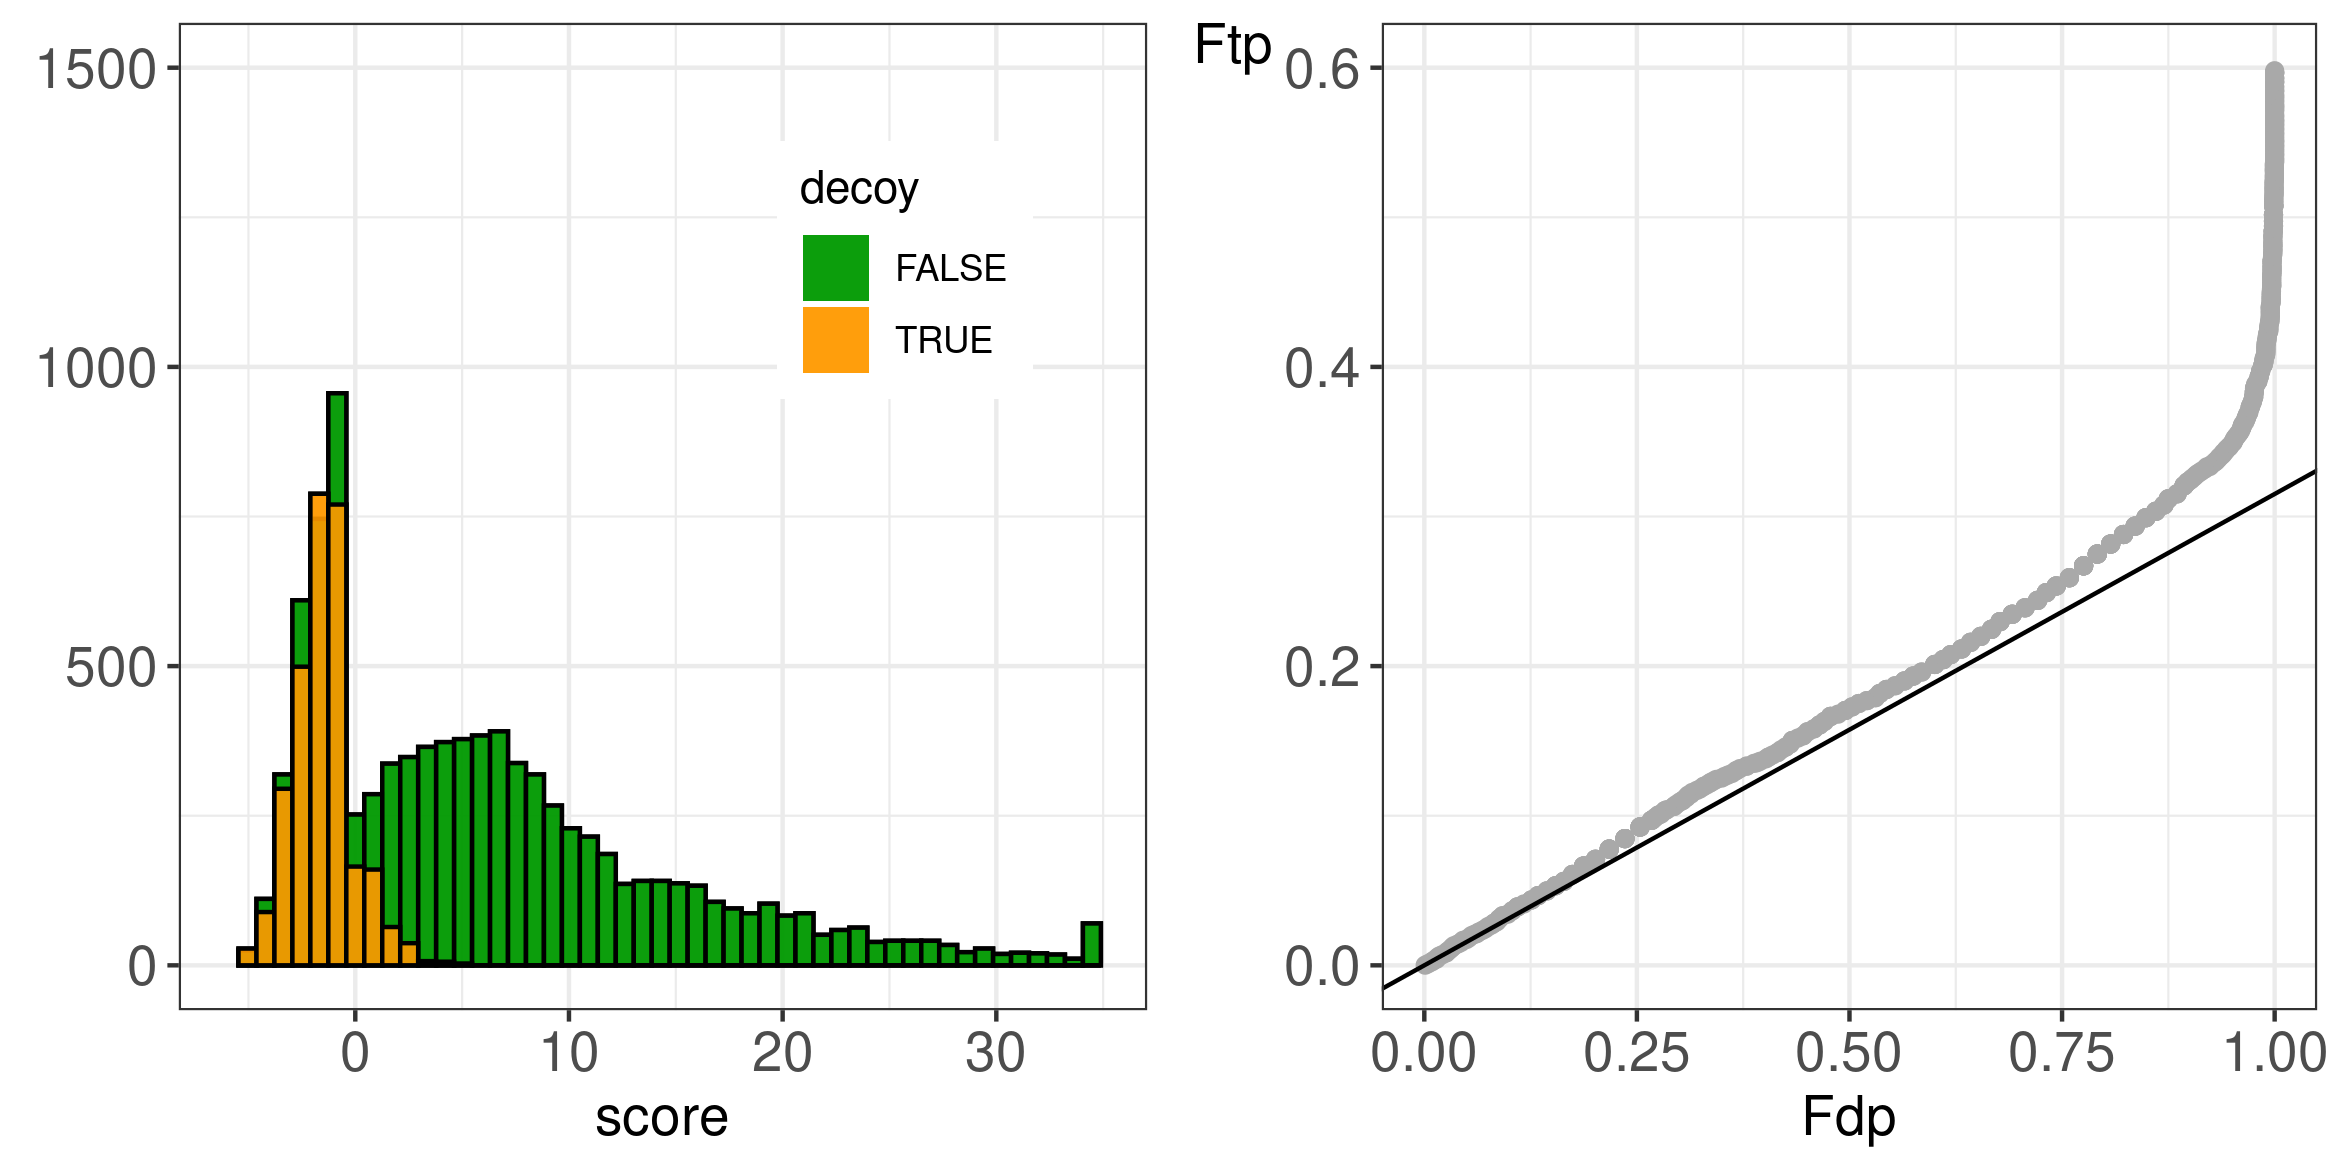
\includegraphics[width=0.99\linewidth]{./figs/figTandemNoRefineSwissHistPP} \caption{Histogram and PP-plot for a concatenated search on a \emph{Pyrococcus} run against a database of canonical \emph{P. furiosus} sequences from Swiss-Prot using X!Tandem without refinement. Both the histogram and the P-P plot show no violation of the TDA assumptions.}\label{fig:sFig1}
\end{figure}



\begin{figure}
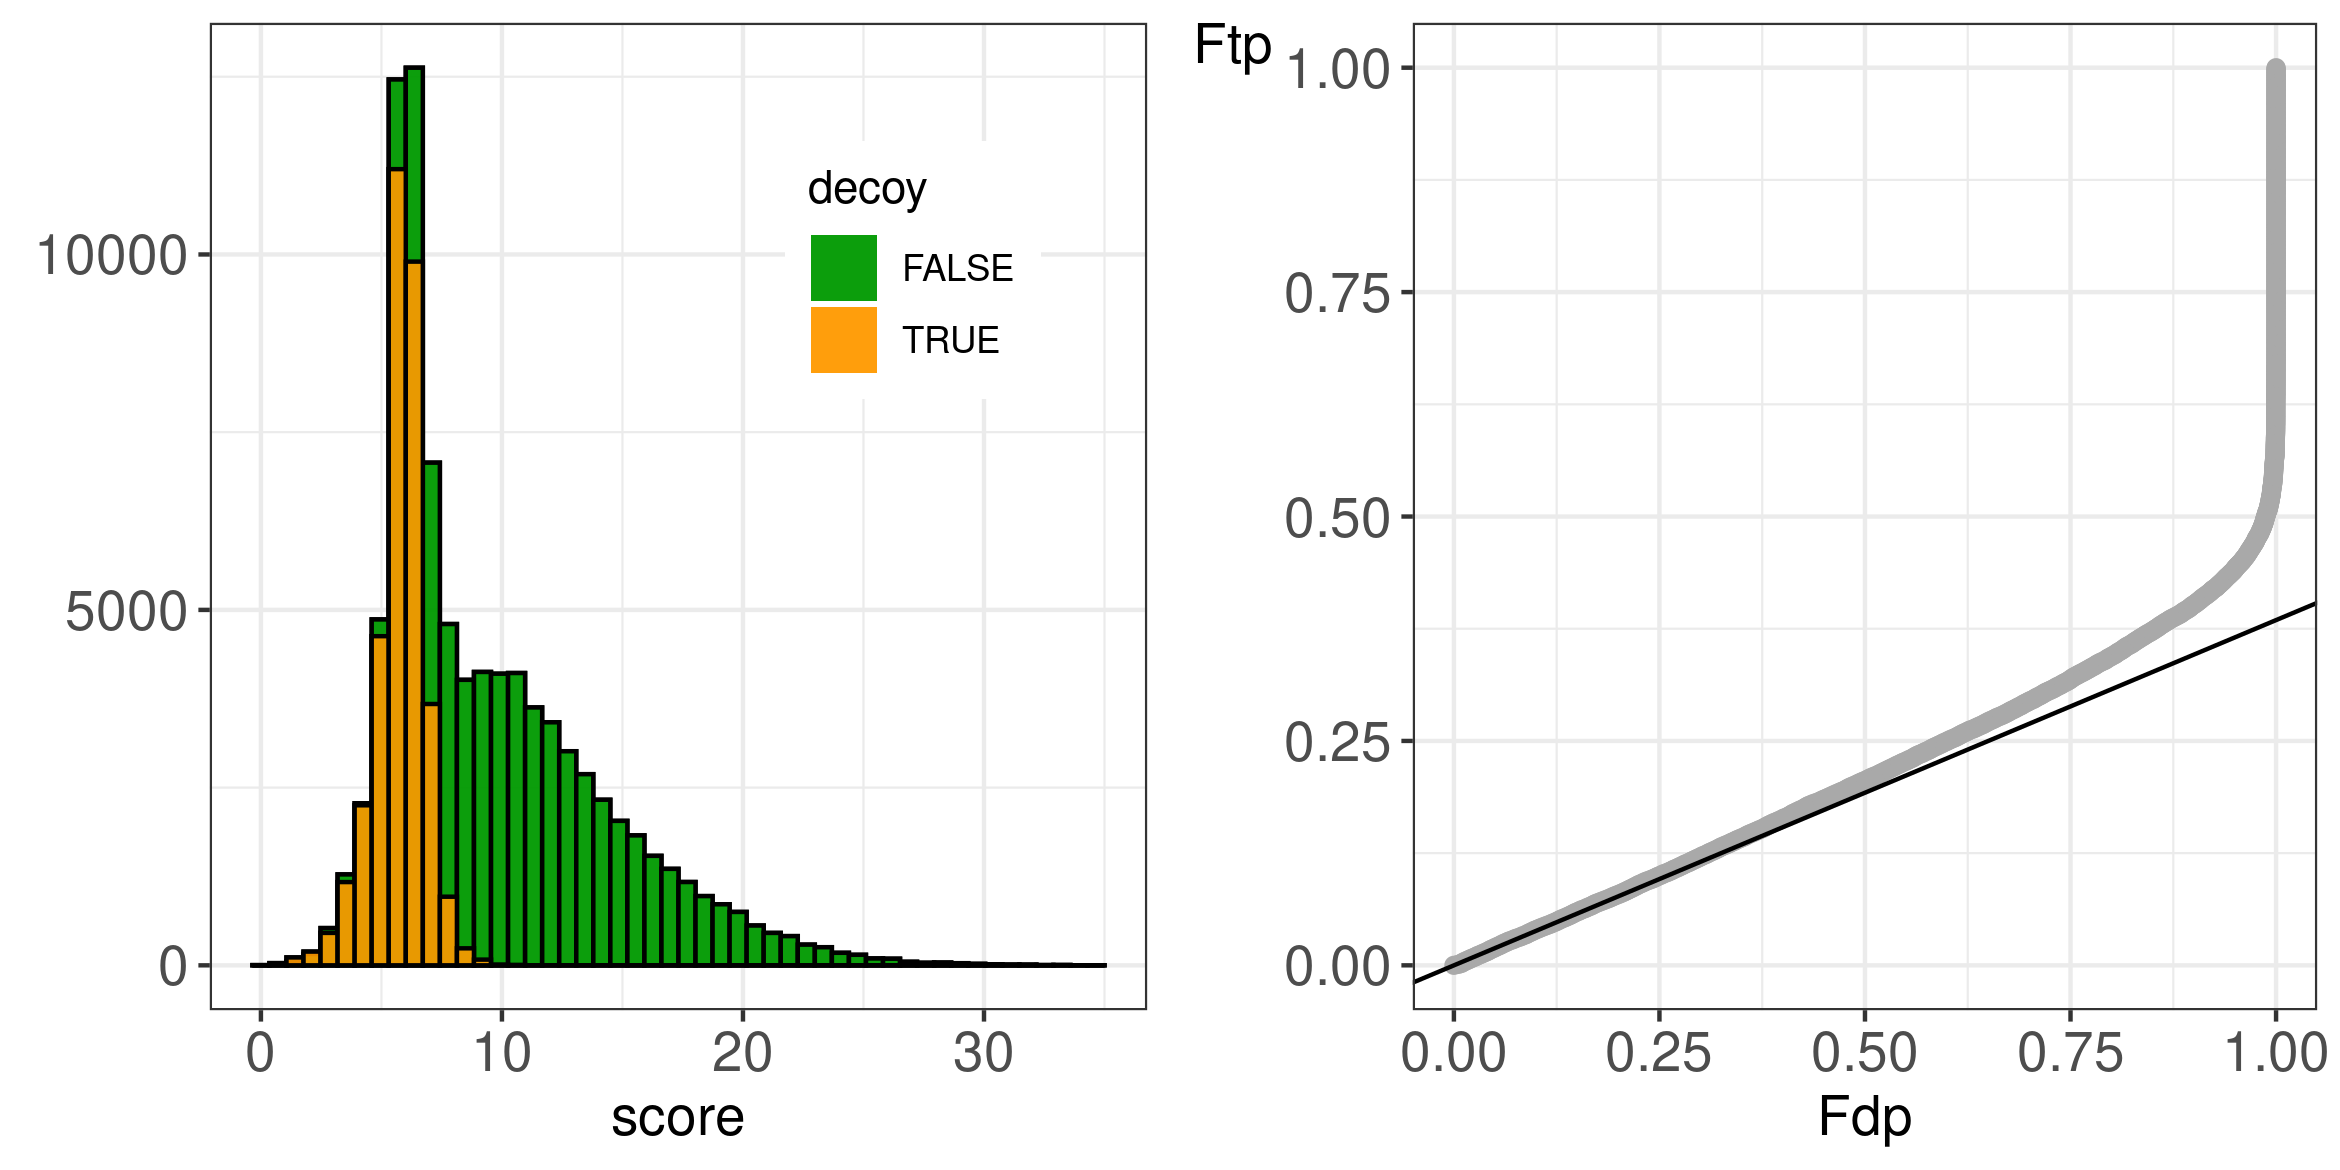
\includegraphics[width=0.99\linewidth]{./figs/figHumanMsgfPlus} \caption{Histogram and PP-plot for a concatenated search on a \emph{H. sapiens} run against a database of \emph{H. Sapiens} sequences from UniProt using MS-GF+. Both the histogram and the P-P plot show no violation of the TDA assumptions.}\label{fig:sFig2}
\end{figure}



\begin{figure}
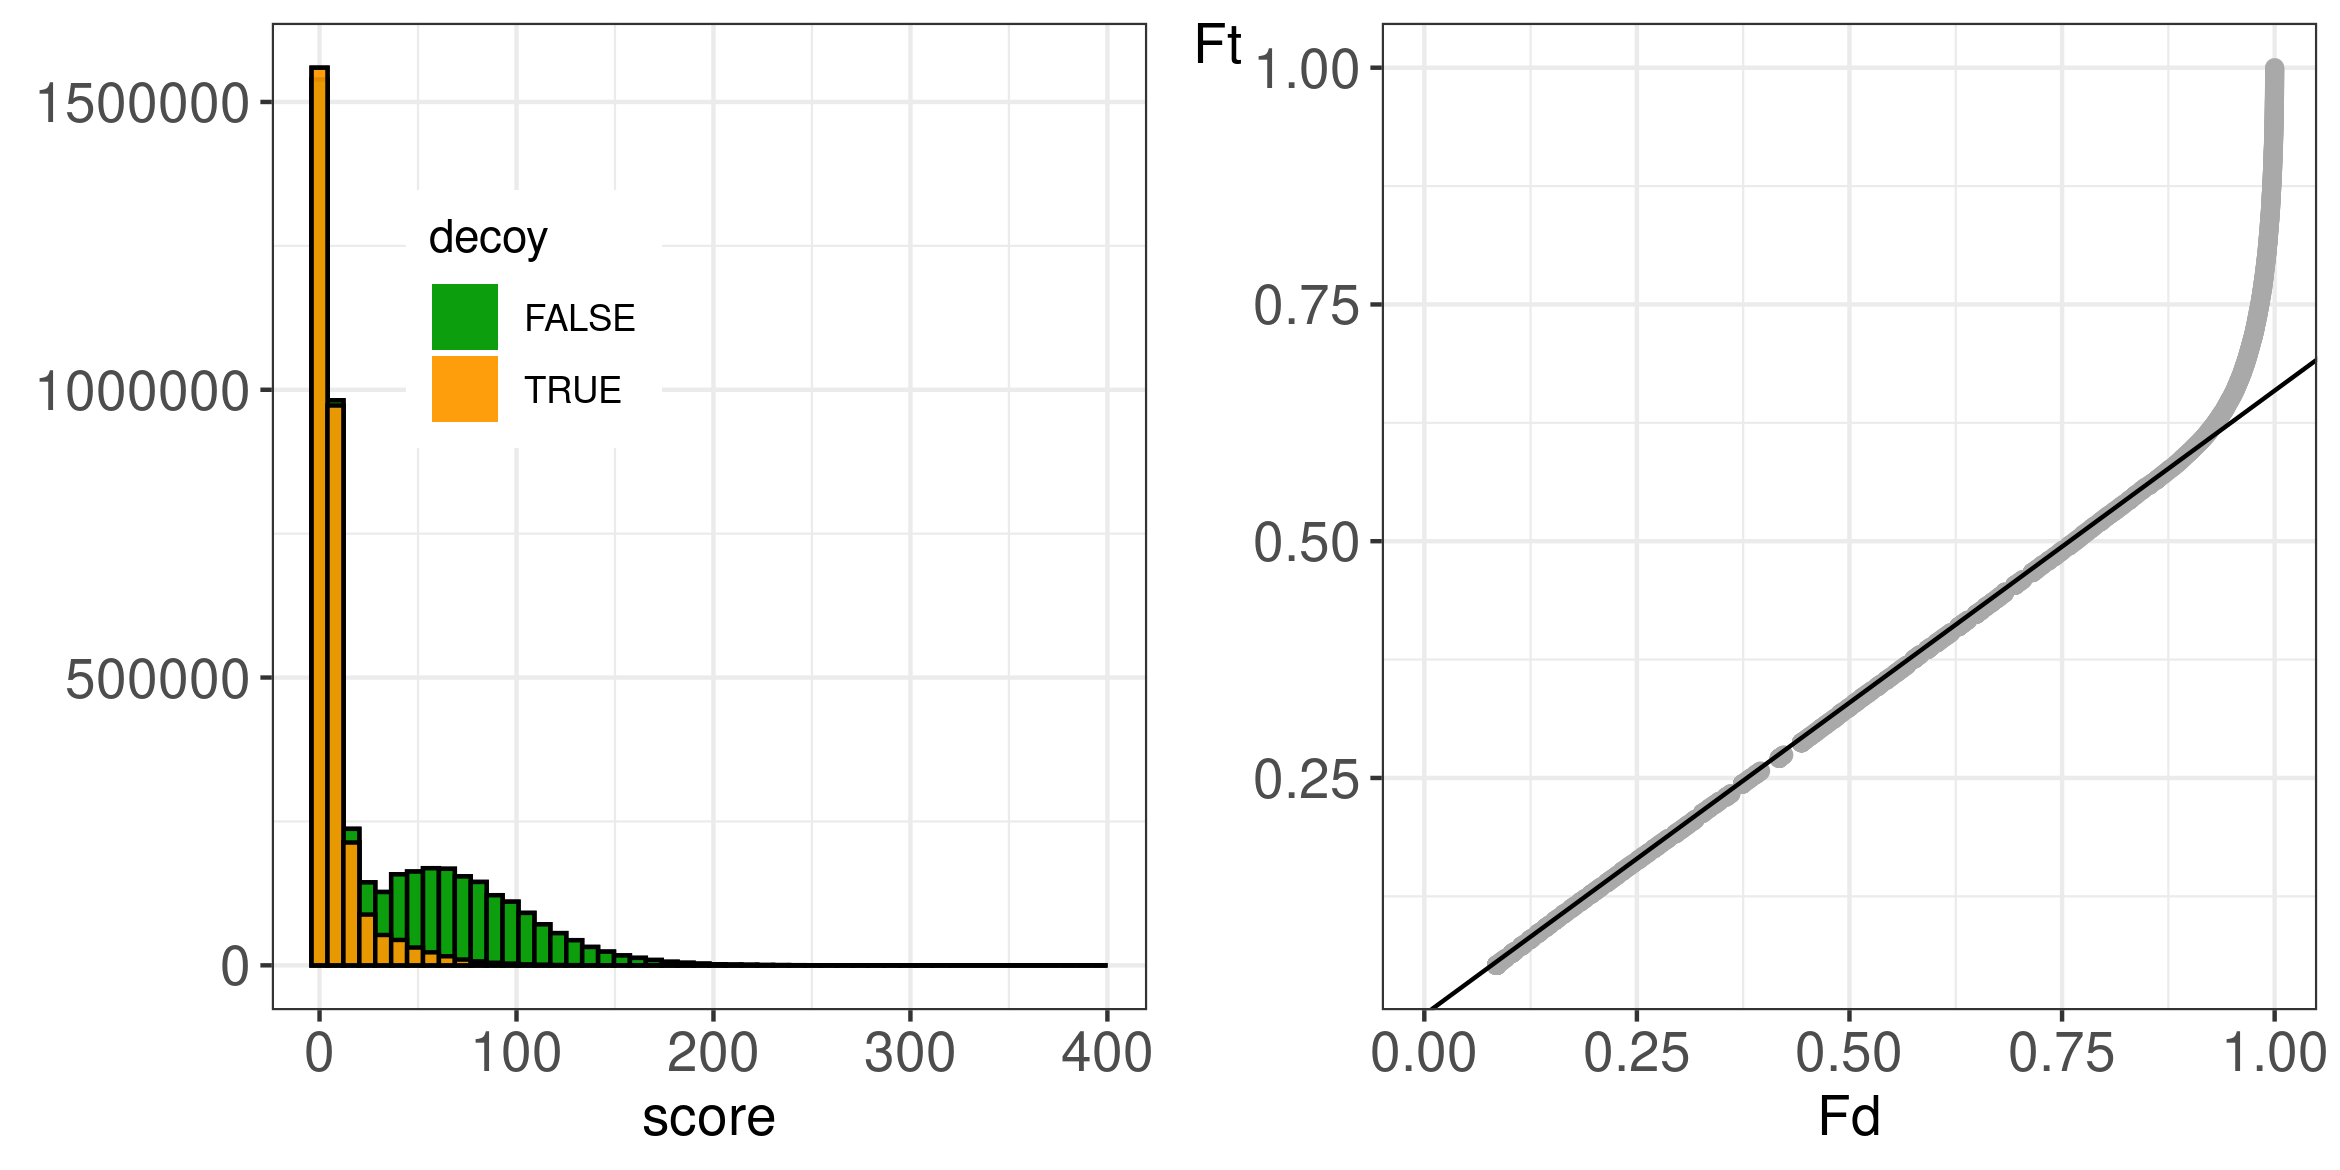
\includegraphics[width=0.99\linewidth]{./figs/figPeptidomics} \caption{Histogram and PP-plot for a concatenated search on an immunopeptidomics run using Andromeda. Both the histogram and the P-P plot show no violation of the TDA assumptions.}\label{fig:sFig3}
\end{figure}



\begin{figure}
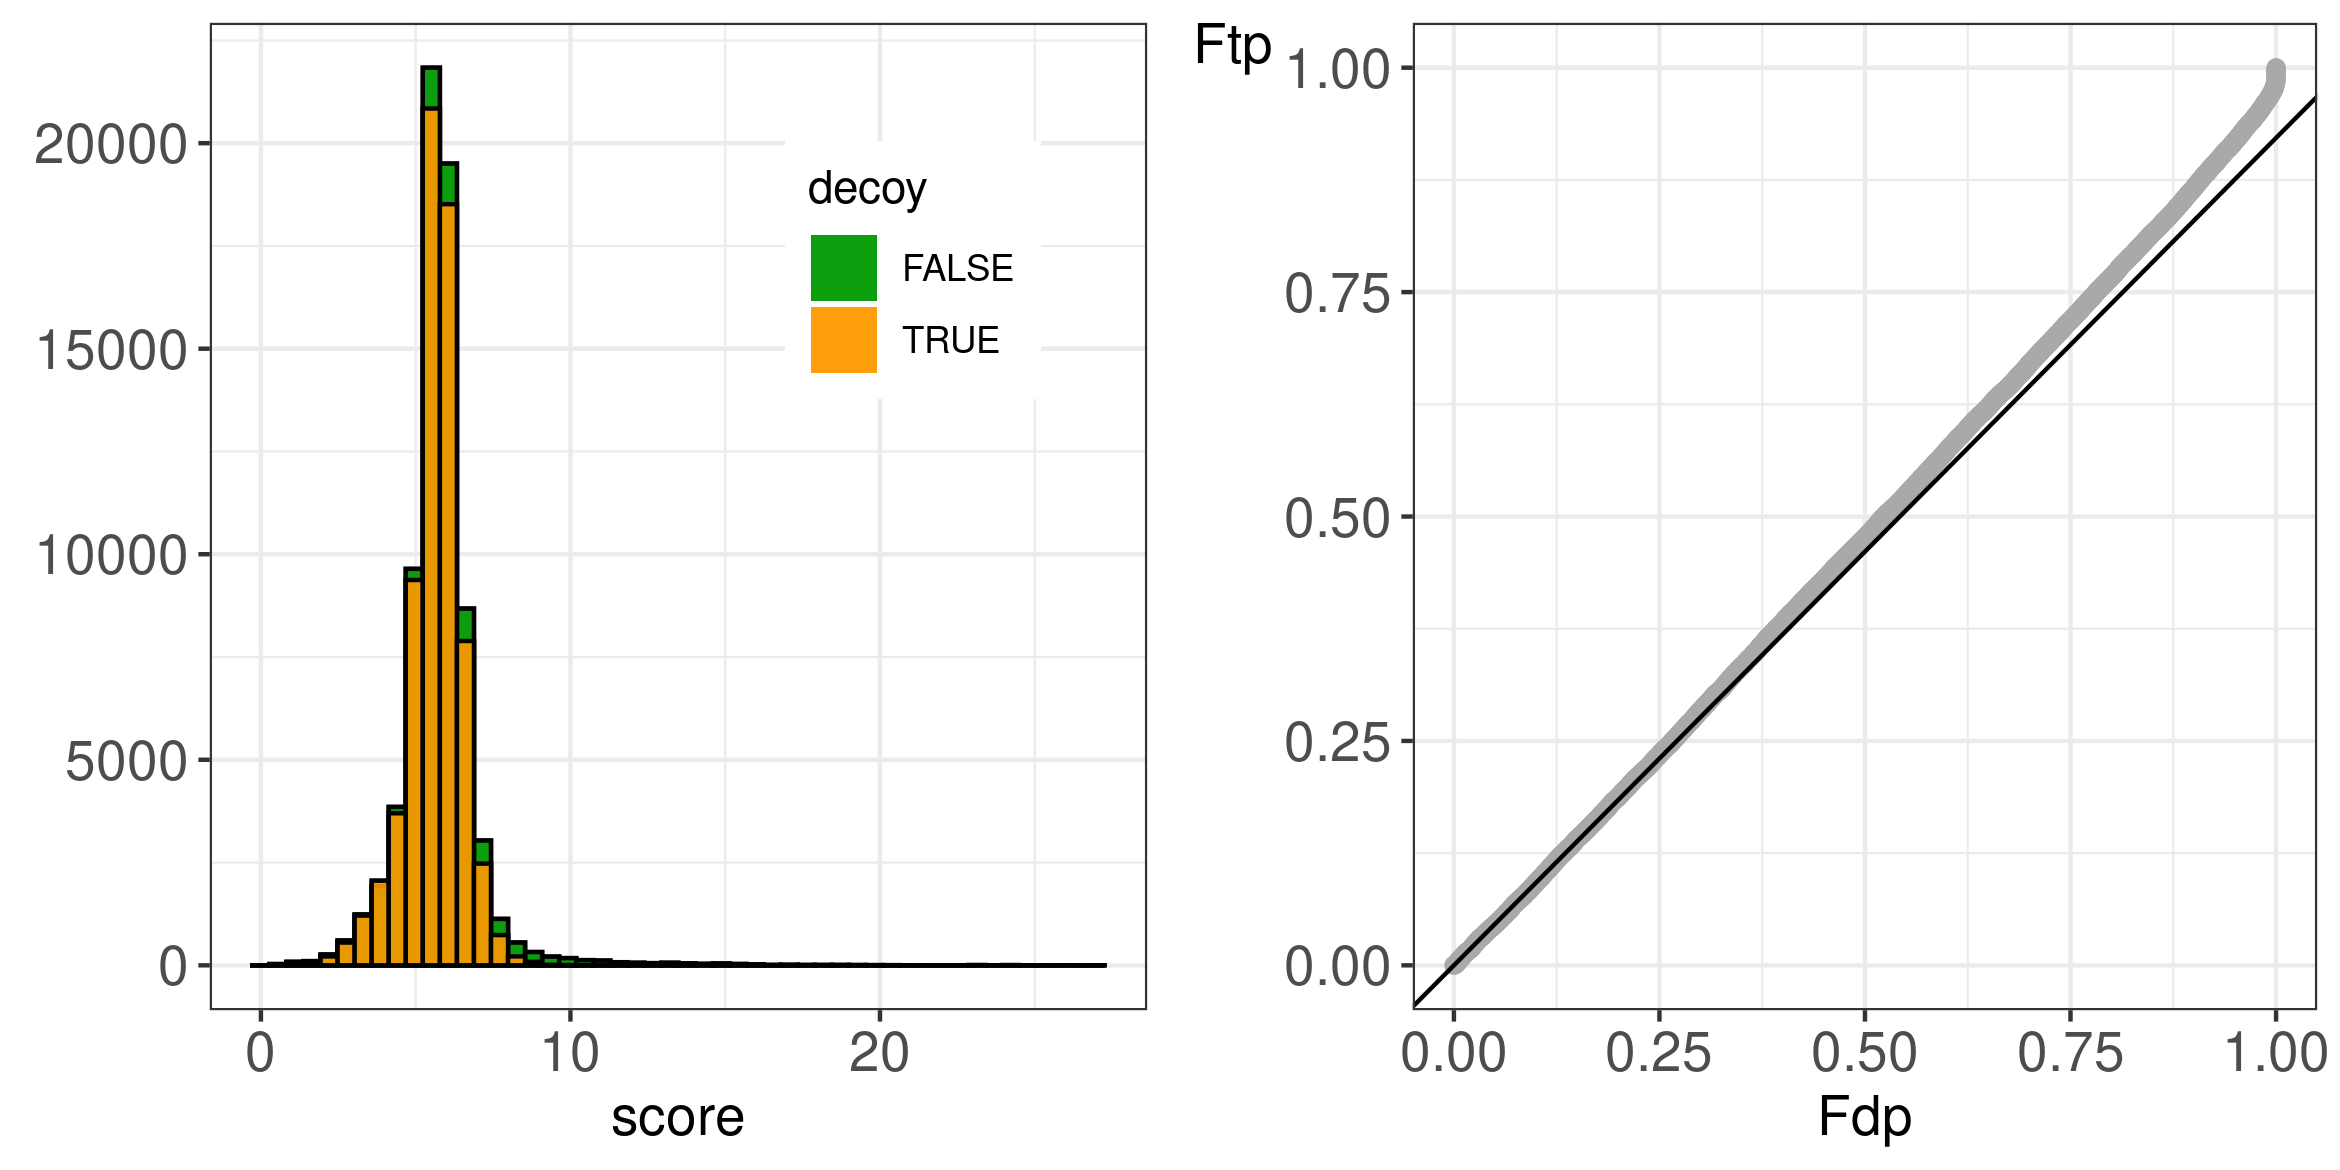
\includegraphics[width=0.99\linewidth]{./figs/figHumanMsgfPlusR2} \caption{Histogram and PP-plot for rank 2 target and decoy PSM scores of a concatenated search on a H. sapiens run against a database of H. Sapiens sequences from UniProt using MS-GF+.}\label{fig:sFig4}
\end{figure}